\documentclass[a4paper,11pt,twoside]{article}
\usepackage[left=2.5cm,right=2cm,top=2cm,bottom=2cm]{geometry}

\usepackage{multirow}
\usepackage[table,xcdraw]{xcolor}
\usepackage{graphicx}
\usepackage{booktabs}
\usepackage{rotating}
\usepackage{epsfig}
\usepackage{amssymb}
\usepackage{amsmath}
\usepackage{amsfonts}
\usepackage{amsthm}
\usepackage{amsmath}
\usepackage{mathtools}
\usepackage{hyperref}

\newcommand{\HRule}{\rule{\linewidth}{0.4mm}}

\setlength{\parindent}{0em}
\setlength{\parskip}{0.5em}

\begin{document}
\begin{center}
  \textbf{\LARGE Inferring Infection Times using Serological Data}\\[.5cm]
  \textbf{\Large Proposal}\\[.5cm]
\end{center}

\section{Introduction}
Serological studies and reporting of influenza like illness (ILI) are the two primary means of assessing influenza infection attack rates. In the former case, blood samples are collected before and after an epidemic, enabling the comparison of serum antibody levels before and after a period of possible infection as measured by a hemagglutination-inhibition titre (HAI) or neutralisation titre (NI). Typically, a 4-fold rise is considered indicative of infection (seroconversion), whilst a 2-fold rise is considered insufficient evidence for infection due to the possibility of measurement error from either sample. In the latter case, reported ILIs during an epidemic give a good idea of the number and timing of infections and may be combined with measures of seroconversion or molecular confirmation of virus infection (rtPCR).

Serological data is particularly appealing for the assessment of infection attack rates for a number of reasons. Firstly, it captures those individuals that might be infected by the virus and not display symptoms. Furthermore, assessing titres against a panel of influenza strains allows us to distinguish between infections with co-circulating strains, which might all present with the same symptoms. Despite these advantages, using serological data comes with a number of complications:

\begin{enumerate}
\item Boosting of antibodies that provide cross-reactive protection may suggest seroconversion in the absence of infection
\item Measurement error from either sample may falsely suggest boosting (false positives), or may miss seroconversion (false negatives) [V1 vs. V2 scatterplots]
\item The 4-fold rise criteria for seroconversion may miss those individuals that have been infected but only receive a modest boost to antibody levels [Simon Cauchemez paper]
\item Sparse longitudinal data make it difficult to infer exact times of infection or temporal dynamics of antibody kinetics
\end{enumerate}

\section{Aims}
We attempt to address these issues by combining data from the FluScape serological survey with a multiple infection model of antibody kinetics. Our model has previously been used the context of assessing antibody kinetics in a cohort of ferrets with known, varied exposure histories. By fitting this model using a Bayesian framework, we hope to estimate infection times for each individual in the presence of measurement error and multiple co-circulating strains. In particular, we hope to address the following questions:
\begin{enumerate}
\item Can we accurately re-capture infection times from a simulated dataset with known, deterministic antibody kinetics?
\item Can we re-capture parameters controlling antibody kinetics in addition to infection times from simulated data?
\item For the above two questions, is the model able to accurately recover simulated parameters in the presence of cross-reactive antibodies to multiple circulating strains? It is the case of multiple infections that accounts for cross-reactivity that is particularly interesting here.
\item How well does our model perform in accounting for and capturing measurement error in observed data? How do we characterise this error (eg. Gaussian, custom measurement error matrix), and can we infer relevant parameter values for this error?
\item Does the incorporation of surveillance data (eg. ILI, epicurves) improve parameter inference, and how can we incporate this data? For example, as a prior for infection time inference.
\item Finally, how well does our model perform in capturing individual infection times and process parameters from the FluScape data?
\end{enumerate}

\section{Methodology}
\subsection{Data}
To test the applicability of our model, we will attempt to recapture known parameter values from simulated data:
\begin{enumerate}
\item HAI titres are taken at two time points - baseline (t0) and t1. It may also be interesting to consider a third time point, t2. That is, each individual will have a log HAI titre against each strain at t0, t1 and t2.
\item In the first instance, we consider only a single circulating influenza strain, and that HAI titres are only performed against this one strain. We will go on to consider three ciruculating strains that may cross-react (H3N2, H1N1, H5N1/H7N9/H9N2).
\item We assume a known epidemic curve for incidence of infection over time. Initially, this might be a uniform distribution over the study period such that everyone is infected at some point. This may then be adapted to be more realistic (eg. an SIR-shaped curve). We will also consider that individuals may or not be infected during the study period.
\item After infection, the antibody levels of each individual undergos a boost and subsequent wane as described by the multiple-infection boosting and waning model. We will assume that these parameters apply to the entire population (ie. one value of $mu$ for each infection). [Do we want to consider process stochasicity? eg. boosting is drawn from a Poisson]
\item Each individual will therefore have a series of true antibody levels over period of the study. We then assume that observations are taken for each individual at t0, t1 and t2. We will incorporate observation error at this point with known dispersion parameters.
\end{enumerate}

We will then apply then attempt to infer infection times and process parameter values from the FluScape data, which consists of a panel of antibody titres to a number of strains at two visits. We will use incidence of ILI over the study period as priors for the infection times.\\

Our force of infection priors will come from weekly incidence of influenza (by subtype) from the WHO website (eg. \url{http://gamapserver.who.int/gareports/Default.aspx?ReportNo=1})\\

\begin{figure}[h!]
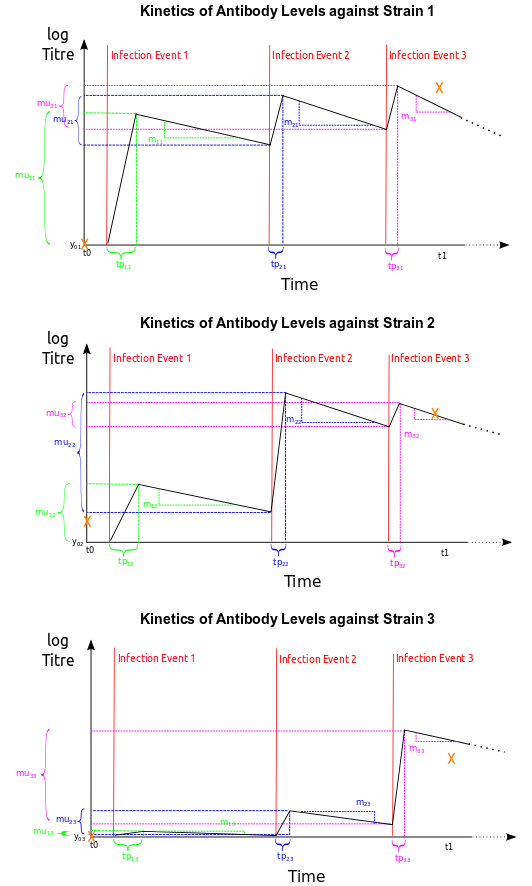
\includegraphics[scale=0.7]{model_cartoon.png}\\
\caption{Cartoon representation of the multiple-infection boosting/waning model. Vertical red lines represent times of infection events; orange crosses represent titre readings; other parameters are as described in the below text.}
\end{figure}

\subsection{Model}
Figure 1 provides a cartoon representation of the model. For each individual, we are concerned with the kinetics of antibodies produced against each strain over the study period. We assume that each infection provides an infection/strain-combination specific cross-reactive boost to antibody levels against all strains, followed by an infection/strain specific waning rate. That is, after an infection from strain $k$ at time $ti_k$, levels of antibodies to strain $j$ are boosted by a set amount ($\mu_{(k,j)}$) $tp_{(k,j)}$ days after the infection, at which point levels begin to wane at a rate $m_{(k,j)}$ log titre units per day. Note that initial antibody levels may not start at 0 the time of infection, and are therefore given by $y_{0_{(k,j)}}$. Prior to the first infection, this value is likely to be 0. For each subsequent infection, initial antibody for a particular infecting strain, $k$, are given by:
\begin{equation}
 y_{0_{(k,j)}}=\left\{
\begin{array}{lr}
0 & k \leqslant 1\\\\
m_{(k-1)}(ti_{(k-1)}+tp_{(k-1)}-ti_k)+\mu_{(k-1)} & else
\end{array}
\right.
\end{equation}

Therefore, for an individual with an infection history of $(ti_k)_{(k=1)}^n$, where $n$ is the total number of infections and $ti_k$ is the time of infection with strain $k$, the kinetics of antibodies against strain $j$ are given by:

\begin{equation}
y(t, j) = \left\{
\begin{array}{lr}
y_{0_{(1,j)}} & t \leqslant ti_1\\\\
\frac{\mu_{(1,j)}}{tp_{(1,j)}}t-\frac{\mu_{(1,j)}}{tp_{(1,j)}}ti_1 + y_{0_{(1,j)}} & ti_1 < t \leqslant ti_1 + tp_{(1,j)}\\\\
-m_{(1,j)}t + m_{(1,j)}(ti_1+tp_{(1,j)})+\mu_{(1,j)}+y_{0_{(1,j)}} & ti_1+tp_{(1,j)} < t \leqslant ti_2\\\\
\frac{\mu_{(2,j)}}{tp_{(2,j)}}t-\frac{\mu_{(2,j)}}{tp_{(2,j)}}ti_2 + y_{0_{(2,j)}} & ti_2 < t \leqslant ti_2 + tp_{(2,j)}\\\\
-m_{(2,j)}t + m_{(2,j)}(ti_2+tp_{(2,j)})+\mu_{(2,j)}+y_{0_{(2,j)}} & ti_2+tp_{(2,j)} < t \leqslant ti_3\\\\
\vdots\\\\
\frac{\mu_{(n,j)}}{tp_{(n,j)}}t-\frac{\mu_{(n,j)}}{tp_{(n,j)}}ti_n + y_{0_{(n,j)}} & ti_n < t \leqslant ti_n + tp_{(n,j)}\\\\
-m_{(n,j)}t + m_{(n,j)}(ti_n+tp_{(n,j)})+\mu_{(n,j)}+y_{0_{(n,j)}} & ti_n+tp_{(n,j)} < t
\end{array}
\right.
\end{equation}

Where $y_{0_{(k,j)}}$ is the titre of antibodies against strani $j$ at the time of infection with strain $k$; $\mu_{(k,j)}$ is the level of boosting of antibodies to strain $j$ elicited following infection with strain $k$; $tp_{(k,j)}$ is the time at which this boost peaks; and $m_{(k,j)}$ is the rate at which is boost wanes.

As each strain potentially provides a cross-reactive boost to each other strain under consideration, it is helpful to think about each of these parameters as coming from an $n$ by $n$ matrix, where $n$ is the total number of strains under consideration.

\subsection{Parameter Inference}
We will use Markov chain Monte Carlo with a Metropolis-Hastings random walk algorithm to estimate univariate posterior distributions for all parameters. In the simplest case where boosting, waning and error parameters are assumed to be known, fitting the model to each individual can be considered independently. In this case, each individual has only three individual-specific parameters: $ti_1$, $ti_2$ and $ti_3$. We can therefore infer estimates for these three parameters separately for each individual ie. we explore the multivariate posterior distribution of $(ti_k)_{k=1}^{n=3}$ conditional on the HI titre data for those three strains.

Once we move onto the case where the boosting and waning parameters are also considered to be unknown, things get a bit trickier. The posteriors for boosting/waning parameters ($mu$,$m$ and $tp$) will be conditional on data for all of the individuals. We will therefore have to implement a Metropolis-Hastings algorithm that block-updates either infection times, boosting/waning parameters or sensitivity/error parameters. In the case of infection times, the number of updated individuals at each step may be varied to affect the acceptance rate.

\begin{enumerate}
\item Likelihood Function: the likelihood for a single observation is the probability of observing that point (discretised gaussian, poisson etc) given the model parameters. We take the log sum over all observations to give the likelihood.
\item Priors: boosting and waning parameters will be given uniform (ie. uninformative) priors. Priors for infection times from a given strain will be given as the density of incidence of ILI over the study period (or confirmed infections).
\item Proposals: in the simple case of only considering infection times for each individual, these can be updated randomly and with a uniform proposal distribution. However, when be consider boosting/waning parameters and error parameters, we will need to block-update these parameters. It would be sensible to use a multivariate-normal proposal for the boosting/waning parameters, whereas the a uniform or univariate gaussian proposal would be sufficient for the infection times.
\end{enumerate}

\subsection{Further Work}
There are a number of ways in which this work might be extended further in the context of the FluScape data:

\begin{enumerate}
\item Using inferred infection times, is it possible to combine this data with spatial data to reconstruct transmission trees? Or is it possible to identify where and when localised outbreaks occured?
\item Incorporation of age or demographic data? eg. boosting and waning parameters specific to certain age groups?
\item Inferred infection times allow us to build an ``epicurve''. We could then fit, say, an SIR model to this curve to recover further epidemiological parameters (eg. R0).
\item As an alternative to considering infection/strain specific parameters (ie. $mu_{(k,j)}$), we might consider the case where all strains have a set boost and waning rate, but the impact of cross-reactivity is mediated by some proportional reduction parameter (eg. $\alpha_{(k,j)}$ is the level of cross-reactivity between strains $j$ and $k$, perhaps defined as antigenic similarity). Similarly, we might consider a binary parameter indicating whether or not an individual has been infected.
\end{enumerate}

\section{Plan}
I propose the following sequence of work:

\begin{enumerate}
\item Implement the data-generating process. Given a number of individuals, times of infection (may be specified from an SIR/epidemic curve), measurement times and observation error distribution, generate a mock serosurvey. Allow a variable number of infecting strains to be considered.
\item Assuming that boosting and waning parameters are known, use the MCMC-MH algorithm to find posterior distributions of infection times for \emph{each} individual. Consider the case that all individuals must be infected at some point from t0 onwards. However, these infection times might be after the second observation time, t1, and we can therefore count these individuals as not infected. Try this with uniform priors, or priors of the epidemic curve that was used to generate the data. This should be done for simulated strains.
\item Repeat the above, but assume that boosting and waning parameters are unknown. Leave observation error assumptions fixed.
\item As above, but try gaussian, poisson and simple observation-error matrix likelihoods. Allow these parameters to be estimated.
\item Assess how much difference epicurve priors make by performing each step with uninformative and informative priors.
\item Inference using FluScape data.
\item Assess how well we can recover parameters from simulated data (credible interval sizes) with mock-serosurveys of varying sampling frequency and size.
\item Statistical analysis of inferred infection times alongside spatial data.
\end{enumerate}

I will continue to work with Rcpp and R.

\end{document}
